\section{Data Processing}
\label{sec:data_processing}

\begin{figure}[htbp]
    \centering
    \begin{adjustbox}{max width=\linewidth, center}
        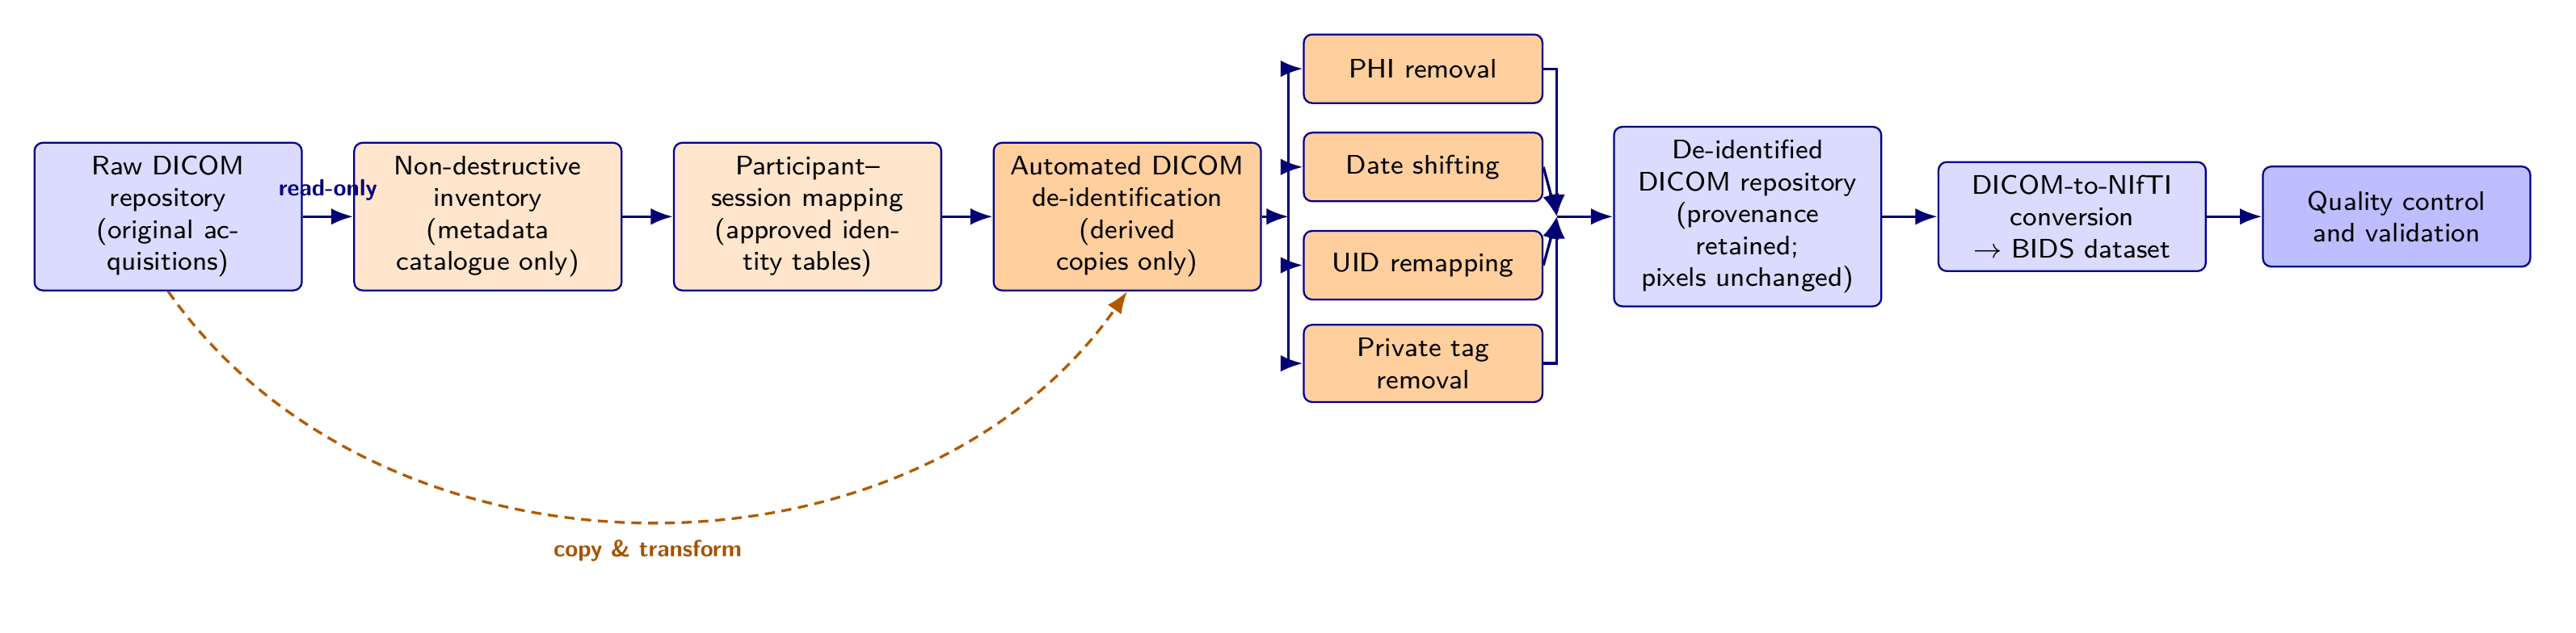
\includegraphics[width=\linewidth]{figures/Figure_2.png}%
    \end{adjustbox}
    \caption{De-identification and release-preparation workflow. Downstream processing uses derived copies; the raw archive is never overwritten.}
    \label{fig:processing_workflow}
\end{figure}

\subsection{DICOM-to-BIDS conversion and dataset construction}
\label{sec:dicom_to_bids}

\subsubsection{DICOM inventory and series identification}

Source DICOM series were inventoried from the original scanner archive without modifying that archive. Each series was assigned pseudonymous BIDS entities---participant label (\texttt{sub-<ID>}), session (\texttt{ses-01} or \texttt{ses-02}), modality folder, and run index---using study mapping tables frozen before conversion. Mapping overrides applied at that stage are documented in \texttt{docs/inventory/MAPPING\_OVERRIDES.md}. Sequence-level coverage and missing families are recorded in \texttt{docs/inventory/}.

\subsubsection{DICOM-to-NIfTI conversion}

De-identified working copies of the DICOM data were converted to gzip-compressed NIfTI with JSON sidecars using \texttt{dcm2niix} (version 1.0.20230411; arguments \texttt{-b y -ba y -z y}). Conversion and BIDS organisation were orchestrated by \texttt{neuro\_pipeline} version 2.1.0, as recorded in \texttt{dataset\_description.json}. After conversion, JSON sidecars were scrubbed of residual personal and institutional identifiers; missing \texttt{TaskName} values were injected from filenames when needed; phase images were renamed to the BIDS \texttt{part-phase} entity; and field-map \texttt{IntendedFor} targets were set where applicable. For Siemens XA30 Enhanced MR sessions in which \texttt{dcm2niix} did not export \texttt{SliceTiming}, values were recovered from DICOM frame timing (\texttt{FrameAcquisitionDateTime} / \texttt{InStackPositionNumber}) when available.

\subsubsection{BIDS organization and naming}

Converted data were organised according to BIDS version 1.9.0 (\texttt{DatasetType}: \texttt{raw}). Imaging files were placed under \texttt{sub-<ID>/ses-<ID>/\{anat,func,dwi,fmap\}/} with standard entities (for example \texttt{task-}, \texttt{run-}, \texttt{dir-AP}/\texttt{dir-PA}, \texttt{part-phase}). Diffusion series include companion \texttt{.bval} and \texttt{.bvec} files. Session-level \texttt{*_scans.tsv} tables list imaging files within each session. Structural compliance of the MRI imaging tree was checked with bids-validator version 1.15.0 (MRI imaging scope; physiology and events documented separately). Remediation preceding the validation snapshot included field-map metadata repairs, filename and entity fixes, XA30 \texttt{SliceTiming} recovery, and inclusion of verified event tables. Remaining validator warnings were reviewed and disclosed rather than suppressed.

\subsection{Diffusion MRI preprocessing}
\label{sec:dwi_preprocessing}

Preprocessed multi-shell diffusion MRI is released under \texttt{derivatives/tractoflow\_normalize\_dwi/} for 66 participants (49 Control and 17 Glaucoma; one session each: \texttt{ses-01}, except \texttt{sub-066}/\texttt{ses-02}). This derivative is the TractoFlow \texttt{Normalize\_DWI} product for the gSlider-SMS acquisitions (\texttt{gsld\_76dir\_b2000\_1mmiso\_AP}), not for the clinical RESOLVE series. Files are named \texttt{sub-<id>\_ses-<id>\_space-dwi\_desc-normalize\_dwi.\{nii.gz,json,bval,bvec\}}. They are analysis-ready derivatives and do not replace the raw BIDS \texttt{dwi/} runs. HCP structural derivatives, fibre-orientation maps, and tractograms are not packaged in this tree.

The raw gSlider volumes retain slab RF encodings (modal geometry $1 \times 1 \times 5$~mm, typically 385 time points, shells $b=0/1000/2000$~s/mm$^2$). Before TractoFlow, gSlider data were reconstructed to 1~mm isotropic diffusion volumes and corrected for $B_1$ inhomogeneity using the turbo-flash $B_1$ maps acquired in the same sessions (\texttt{tfl\_b1map\_1mmiso} / \texttt{TB1TFL}) \cite{liao2020gslider}. Reverse phase-encode $b=0$ gSlider references (\texttt{gsld\_75TE\_PA\_3b0}) were used for susceptibility-distortion correction.

A well-designed pre- and post-processing stream is critical for robust tractography. In the IronTract challenge, replacing candidate preprocessing methods with a top-ranking pipeline improved results \cite{maffei2022irontract}. Diffusion preprocessing therefore used a modified TractoFlow pipeline \cite{theaud2020tractoflow} informed by the IronTract and DiSCo challenges \cite{girard2023disco}. Relative to default TractoFlow, denoising used NORDIC \cite{moeller2021nordic} rather than the standard MP-PCA step, and orientation-distribution-function estimation was updated (those fODF products are not in this release). The stream applied to the volumes packaged here comprised NORDIC denoising, Gibbs-ringing correction \cite{kellner2016gibbs}, and correction for motion, eddy currents, and susceptibility distortions with FSL TOPUP and EDDY \cite{andersson2003topup,andersson2016eddy}, followed by N4 bias-field correction (ANTs), resampling to 1~mm isotropic resolution, and intensity normalization. The released volumes remain in native diffusion space and are not skull-stripped. Each series contains 77 volumes (4 $b=0$, 37 $b=1000$~s/mm$^2$, 36 $b=2000$~s/mm$^2$; 73 unique non-$b=0$ directions). A representative reconstructed matrix is $147 \times 183 \times 145$. TractoFlow also takes a T1-weighted volume; the collaborator QC registered that T1 into diffusion space, but T1/FLAIR anatomy is not duplicated inside \texttt{tractoflow\_normalize\_dwi/}. Visual QC of this derivative is described in Section~\ref{sec:quality_control}.

\subsection{Physiological data processing}
\label{sec:physiology_processing}

Siemens PhysioLog DICOM were converted to BIDS physiology files (\texttt{*_recording-<channel>\_physio.tsv.gz} with matching JSON sidecars) only when release gates were met: usable sampling metadata, a derivable start time relative to the linked BOLD series, and a unique BOLD association. Channels written under this policy are \texttt{pulse}, \texttt{respiratory}, and \texttt{trigger} (ECG was not retained in the packaged tree). Sidecars were restricted to an allowlisted metadata set, including \texttt{SamplingFrequency}, \texttt{StartTime}, \texttt{StartTimeMethod}, and \texttt{StartTimeConfidence}. Failed-gate PhysioLogs and session-wide peripheral PMU logs without unique run linkage were not written into the BIDS tree. Physiology files, when present, are colocated with the corresponding functional run under \texttt{func/}. Absence of physiology for a given run indicates a failed conversion gate or no archived PhysioLog for that acquisition, not an invalid BOLD series. Eye-tracking time series are not included in this release.

\subsection{Event and stimulus metadata processing}
\label{sec:events_processing}

Task event tables were generated from experimental records only when a unique protocol-to-BOLD correspondence could be established. For \texttt{task-fmri}, \texttt{*_events.tsv} files provide \texttt{onset}, \texttt{duration}, and \texttt{trial\_type} (\texttt{baseline} or \texttt{stim-01}--\texttt{stim-12}); onsets were reconstructed from measured scanner trigger recordings combined with stimulus-order metadata, without substituting a default TR or inventing onsets for unmatched runs. Condition definitions are provided in \texttt{code/task-fmri\_condition\_dictionary.tsv} (with JSON sidecar) and dataset-root \texttt{task-fmri\_events.json}; the canonical stimulus script \texttt{code/presentStimParams.m} is released for provenance. For \texttt{task-movie}, design-level events accompany magnitude movie runs and include \texttt{onset}, \texttt{duration}, \texttt{trial\_type}, \texttt{stim\_file}, \texttt{eye}, \texttt{movie\_label}, and \texttt{matlab\_run\_id} (definitions in \texttt{task-movie\_events.json}). Movie timing uses \texttt{onset = 0} under the documented protocol assumption that acquisition and clip playback started together; these events are not millisecond TTL-locked onsets. Copyrighted movie video files are not redistributed. Resting-state and control runs have no event files by design. Event inventories are summarised under \texttt{docs/events/}.

\subsection{De-identification and privacy protection}
\label{sec:deidentification}

DICOM de-identification was applied to mapped working copies before NIfTI conversion; original scanner exports remained an unmodified archive. Header processing followed a custom attribute-confidentiality policy oriented toward the DICOM PS3.15 Basic Application Level Confidentiality Profile (curated tag actions; not claimed as certified full-profile compliance). Direct identifiers were replaced with study codes; institutional, physician, accession, device-serial, and related free-text identifier fields were cleared; private tags were removed except where required for reconstruction metadata; UIDs were deterministically remapped; and calendar dates were shifted by a participant-specific offset while preserving longitudinal intervals. Acquisition parameters required for analysis (including series descriptions) and participant sex were retained by default. Image pixel values were not altered during DICOM header de-identification. After conversion, BIDS JSON sidecars were re-scrubbed and audited for residual forbidden personal or institutional fields. The public \texttt{participants.tsv} is limited to \texttt{participant\_id}, \texttt{cohort}, and \texttt{sex}. Source DICOM is not redistributed. Anatomical facial features on shared T1-weighted and FLAIR volumes were removed with \texttt{pydeface} (version 2.0.0+computecanada) and FSL (version 6.0.7.20); in this package the defaced anatomicals are distributed in the BIDS \texttt{anat/} hierarchy. Identity mapping tables and the per-subject date-shift table are not included. De-identification audits are provided under \texttt{docs/deidentification/}.
